\documentclass[tikz]{standalone}
\usepackage{tikz}
\usetikzlibrary{shapes,arrows}

\tikzstyle{startstop} = [rectangle,rounded corners,minimum width=3cm,minimum height=1cm,align=center,draw=black, text width=2.5cm, fill=green!30]

\tikzstyle{therapy} = [trapezium, trapezium left angle =70, trapezium right angle=110, minimum width=2.5cm, minimum height = 1cm, centered,draw=black,align=center, fill=orange!30]

\tikzstyle{decision} = [diamond, minimum width = 3cm, minimum height = 3cm, text centered, draw=black, text width = 2cm,align=center,fill=blue!30]

\tikzstyle{arrow} = [thick, ->, >=stealth]
\tikzstyle{doublearrow} = [<->, thick, >=stealth]

\begin{document}
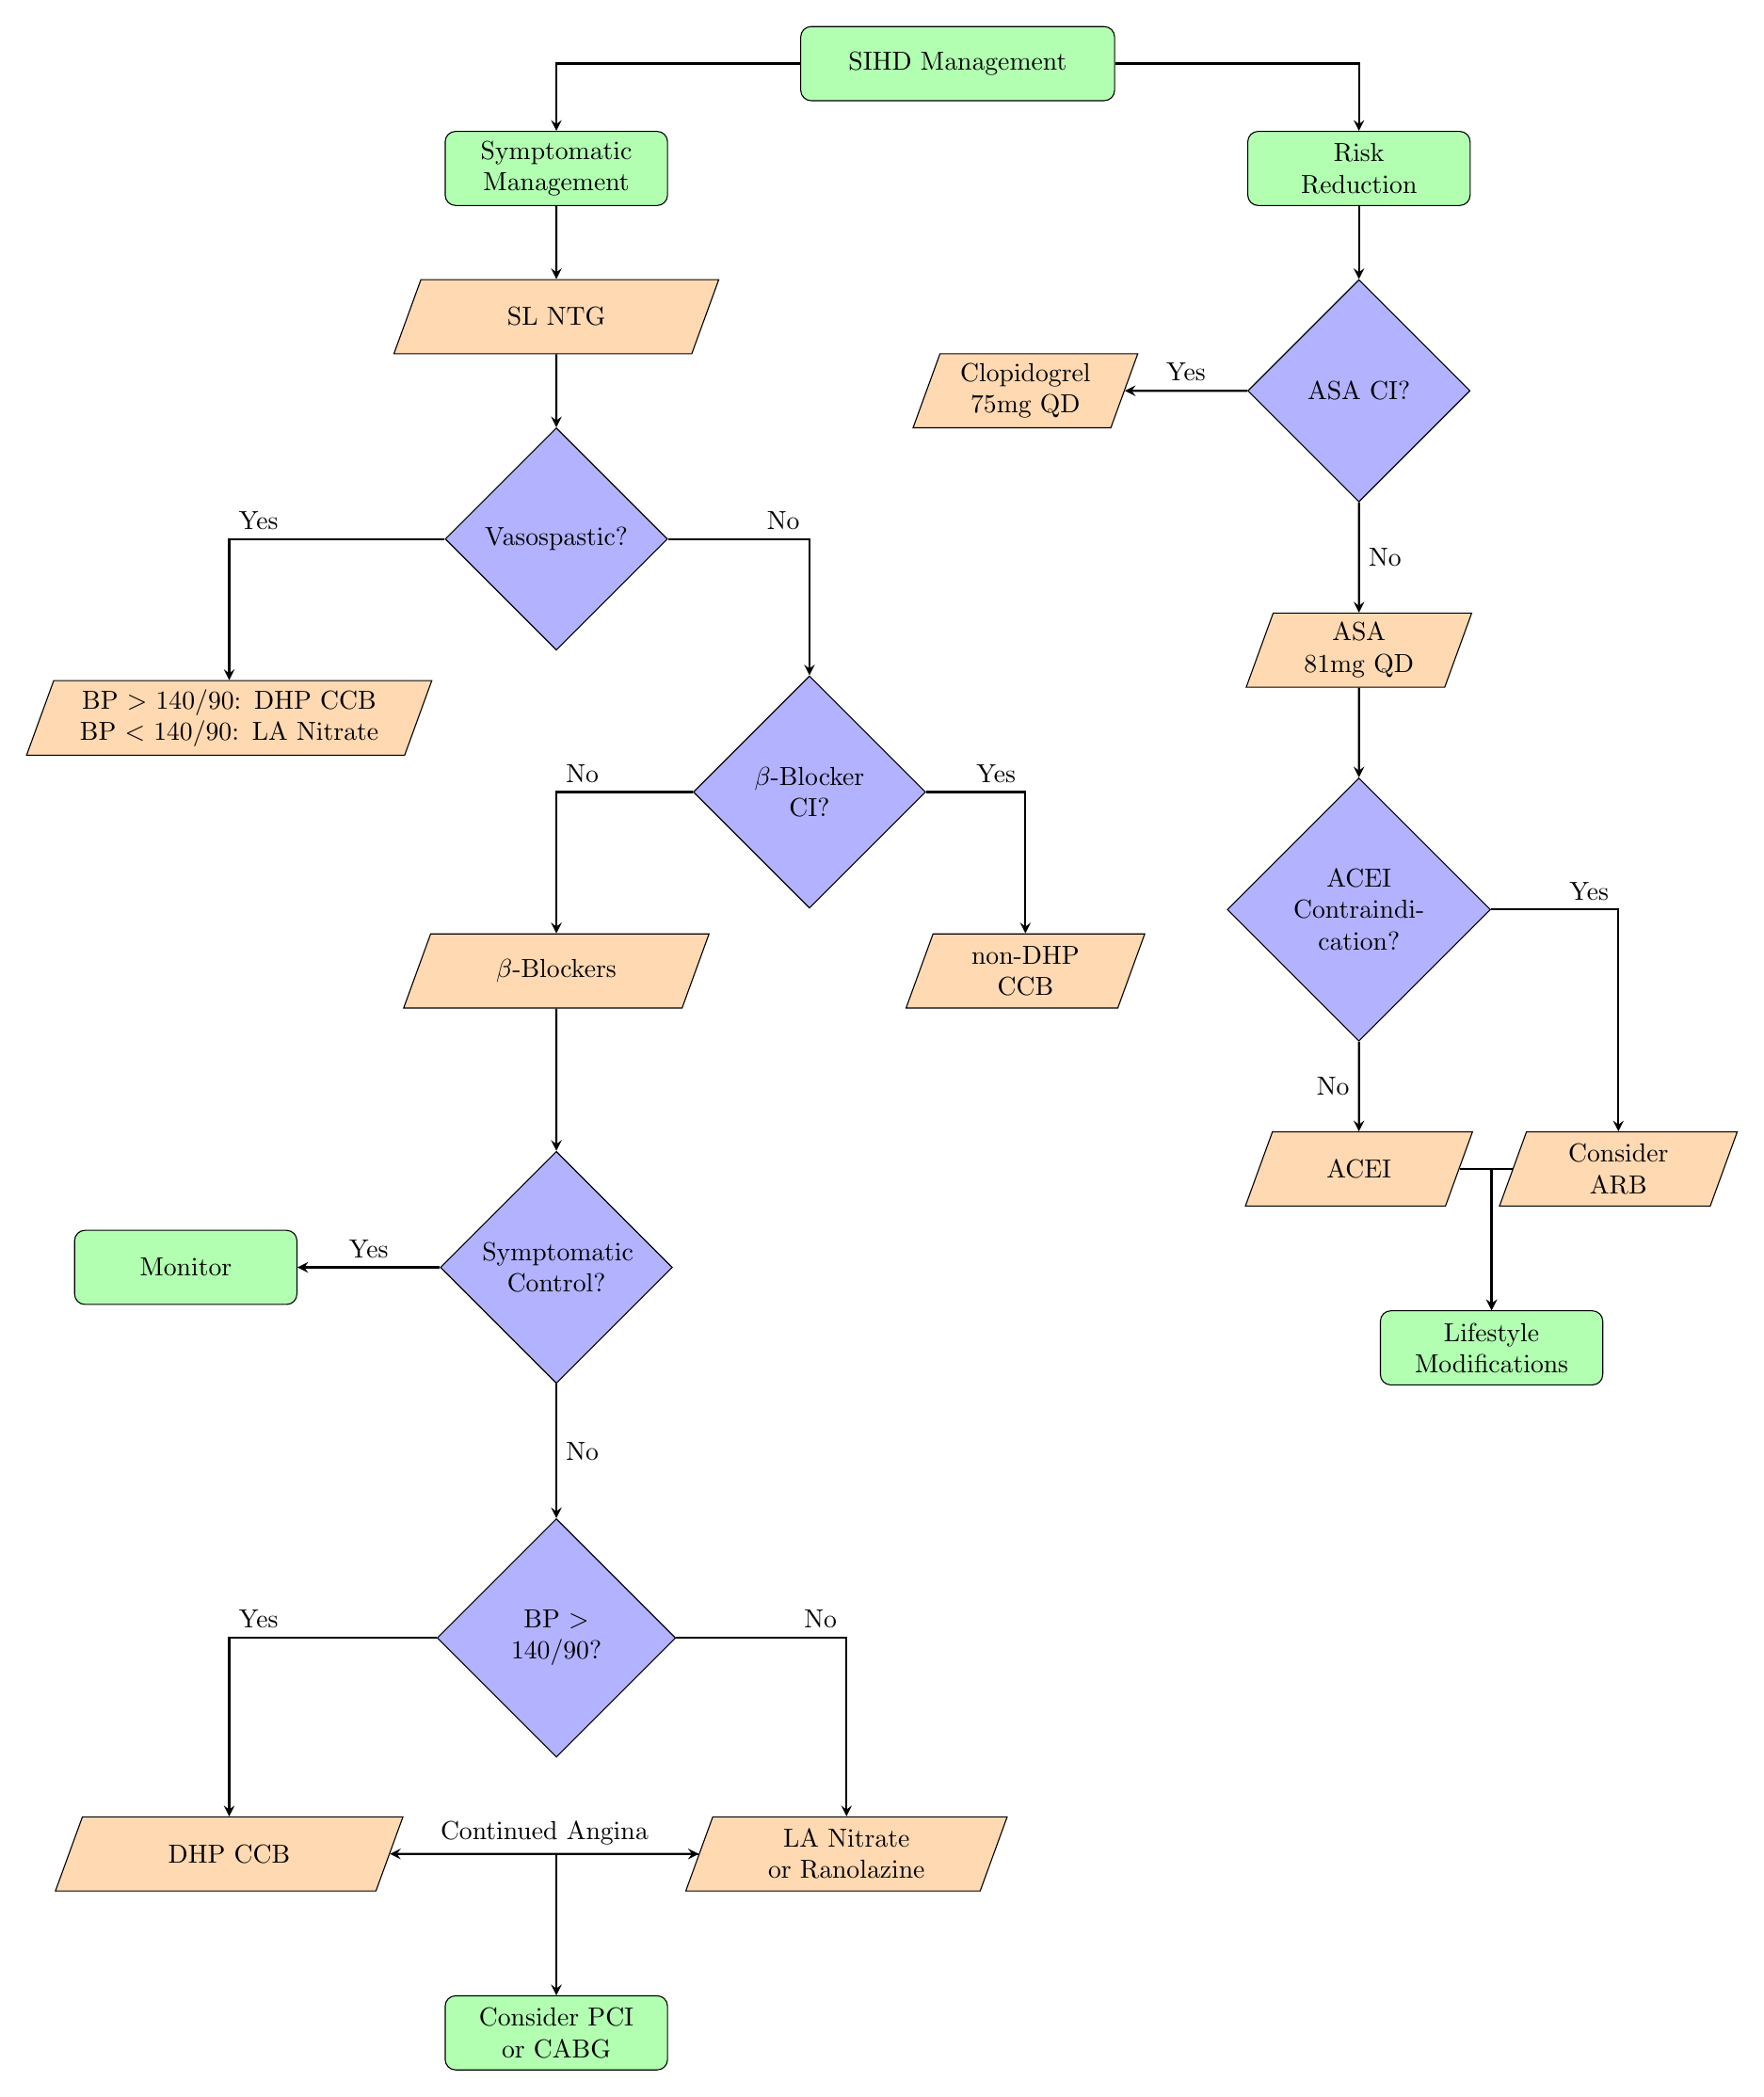
\begin{tikzpicture}[node distance=2cm]

\node (sihd) [startstop, text width=4cm] {SIHD Management};
\node (ssx) [startstop, below left of=sihd,xshift=-4cm] {Symptomatic  Management};
\node (risk) [startstop, below right of=sihd, xshift=4cm,text width = 2cm] {Risk Reduction};
\node (slNTG) [therapy, below of=ssx, text width=1.5cm] {SL NTG};
\node (vaso) [decision, below of=slNTG, yshift=-1cm] {Vasospastic?};
\node (vasospastic) [therapy, below left of=vaso, text width = 4.5cm, xshift = -3cm, yshift=-1cm] {BP $>$ 140/90: DHP CCB BP $<$ 140/90: LA Nitrate};
\node (bbCI) [decision, below right of=vaso, xshift =2cm, yshift=-2cm] {$\beta$-Blocker CI?};
\node (bbs) [therapy, below left of=bbCI, xshift = -2cm, yshift = -1cm] {$\beta$-Blockers};
\node (nonDHP) [therapy, below right of=bbCI, text width=2cm, xshift=1.5cm, yshift = -1cm] {non-DHP CCB};
\node (ssxControl) [decision, below of=bbs, yshift=-2cm] {Symptomatic Control?};
\node (control) [startstop, left of=ssxControl,xshift=-3cm] {Monitor};
\node (bp) [decision, below of=ssxControl, yshift=-3cm] {BP $>$ 140/90?};
\node (dhp) [therapy, below left of=bp,xshift = -3cm, yshift = -1.5cm] {DHP CCB};
\node (nitrate) [therapy, below right of=bp,xshift = 2.5cm, yshift = -1.5cm, text width = 3cm] {LA Nitrate or Ranolazine};
\node (cabg) [startstop, below left of=nitrate, xshift = -2.5cm, yshift=-1cm] {Consider PCI or CABG};

\node (asaCI) [decision, below of=risk, yshift=-1cm] {ASA CI?};
\node (asa) [therapy, below of=asaCI, yshift=-1.5cm, text width = 2cm] {ASA 81mg QD};
\node (clopid) [therapy, left of=asaCI, text width=2cm, xshift = -2.5cm] {Clopidogrel 75mg QD};
\node (aceiCI) [decision, below of=asa, yshift=-1.5cm] {ACEI Contraindication?};
\node (acei) [therapy, below of=aceiCI, yshift=-1.5cm] {ACEI};
\node (arb) [therapy, right of=aceiCI, text width = 2cm, xshift = 1.5cm, yshift=-3.5cm] {Consider ARB};
\node (life) [startstop, below right of=acei, text width = 2.5cm, yshift = -1cm, xshift=0.375cm] {Lifestyle Modifications};




\draw [arrow] (sihd) -| (ssx);
\draw [arrow] (ssx) -- (slNTG);
\draw [arrow] (slNTG) -- (vaso);
\draw [arrow] (vaso) -| node[anchor=south west] {Yes} (vasospastic);
\draw [arrow] (vaso) -| node[anchor=south east] {No} (bbCI);
\draw [arrow] (bbCI) -| node[anchor=south west] {No} (bbs);
\draw [arrow] (bbCI) -| node[anchor=south east] {Yes} (nonDHP);
\draw [arrow] (bbs) -- (ssxControl);
\draw [arrow] (ssxControl) -- node[anchor=south] {Yes} (control);
\draw [arrow] (ssxControl) -- node[anchor=west] {No} (bp);
\draw [arrow] (bp) -| node[anchor=south west] {Yes} (dhp);
\draw [arrow] (bp) -| node[anchor=south east] {No} (nitrate);
\draw [doublearrow] (dhp) -- node[anchor=south] {Continued Angina} (nitrate);
\draw [arrow] (nitrate) -| (cabg);

\draw [arrow] (sihd) -| (risk);
\draw [arrow] (risk) -- (asaCI);
\draw [arrow] (asaCI) -- node[anchor=south] {Yes} (clopid);
\draw [arrow] (asaCI) -- node[anchor=west] {No} (asa);
\draw [arrow] (asa) -- (aceiCI);
\draw [arrow] (aceiCI) -- node[anchor=east] {No} (acei);
\draw [arrow] (aceiCI) -| node[anchor=south east] {Yes} (arb);
\draw [arrow] (acei) -| (life);
\draw [arrow] (arb) -| (life);


\end{tikzpicture}	
\end{document}